\documentclass[conference,11pt,a4paper]{IEEEtran}
\renewcommand\IEEEkeywordsname{Keywords}
\usepackage[utf8]{inputenc}
\usepackage[T1]{fontenc}
\usepackage[english]{babel}

% figures, subfigures, etc.
\usepackage{epsfig}
\usepackage{subfigure}

% equalize the lengths of two columns on the last page
\usepackage{flushend}

% to inser a picture
\usepackage{graphicx}

% abbreviation management
\usepackage[printonlyused]{acronym}

% to incert celsius degrees
\usepackage{textcomp}

% own commands to be used in the draft version
\usepackage[usenames,dvipsnames]{color}
\usepackage[usenames,dvipsnames]{xcolor}

% draft commands
\newcommand{\todo}[1]{\textcolor{red}{\textbf{TODO}: #1}}
\newcommand{\fixme}[1]{\textcolor{BurntOrange}{\textbf{FIXME}: #1}}
%Aramis added
\usepackage{anyfontsize}
%\pagenumbering{roman}
\pagestyle{plain}

\begin{document}
	
	%%%%%%%%%% HEADER %%%%%%%%%%%%%%%%%%%%%%%%%%%%%%%%%%%%%%%%%%%%%%%%%%%%%%
	% Title
	\title{Secure level of RDS Systems}
	% Author
	\author{
		% Author's name
		\IEEEauthorblockN{Juan Aramis Oposich}
		% Author's affiliation
		\IEEEauthorblockA{
			% Author's mail address
			{el17b502@technikum-wien.at}}
	}
	\bstctlcite{IEEEexample:BSTcontrol}
	\maketitle
	\thispagestyle{plain}
	\pagestyle{plain}
	%%%%%%%%%%%%%%%%%%%%%%%%%%%%%%%%%%%%%%%%%%%%%%%%%%%%%%%%%%%%%%%%%%%%%%%%
	
	%%% Introduction %%%
	\section{What is RDS?}
	\textit{Radio Data System} (RDS) is a fast communication standard for FM radio broadcasting. Blaupunkt, a German radio manufacturer, and the European institute for broadcast technology developed a common RDS standard in 1983 \cite{Grds}. This single way communication standard is used to inform hosts about current traffic conditions and music information. Furthermore, navigation systems like Garmin and TomTom use RDS to calculate the quickest path to a destination. FM broadcasting provides five features at nowadays. The features are mono audio, stereo audio, RDS, DirectBand and an audio subcarrier. Figure 1 shows the frequency spectrum of an FM channel with the embedded features \cite{standard}. The bandwidth and the localization of RDS can be determined from the spectrum.
	
	\begin{figure}[h]
		\centering
		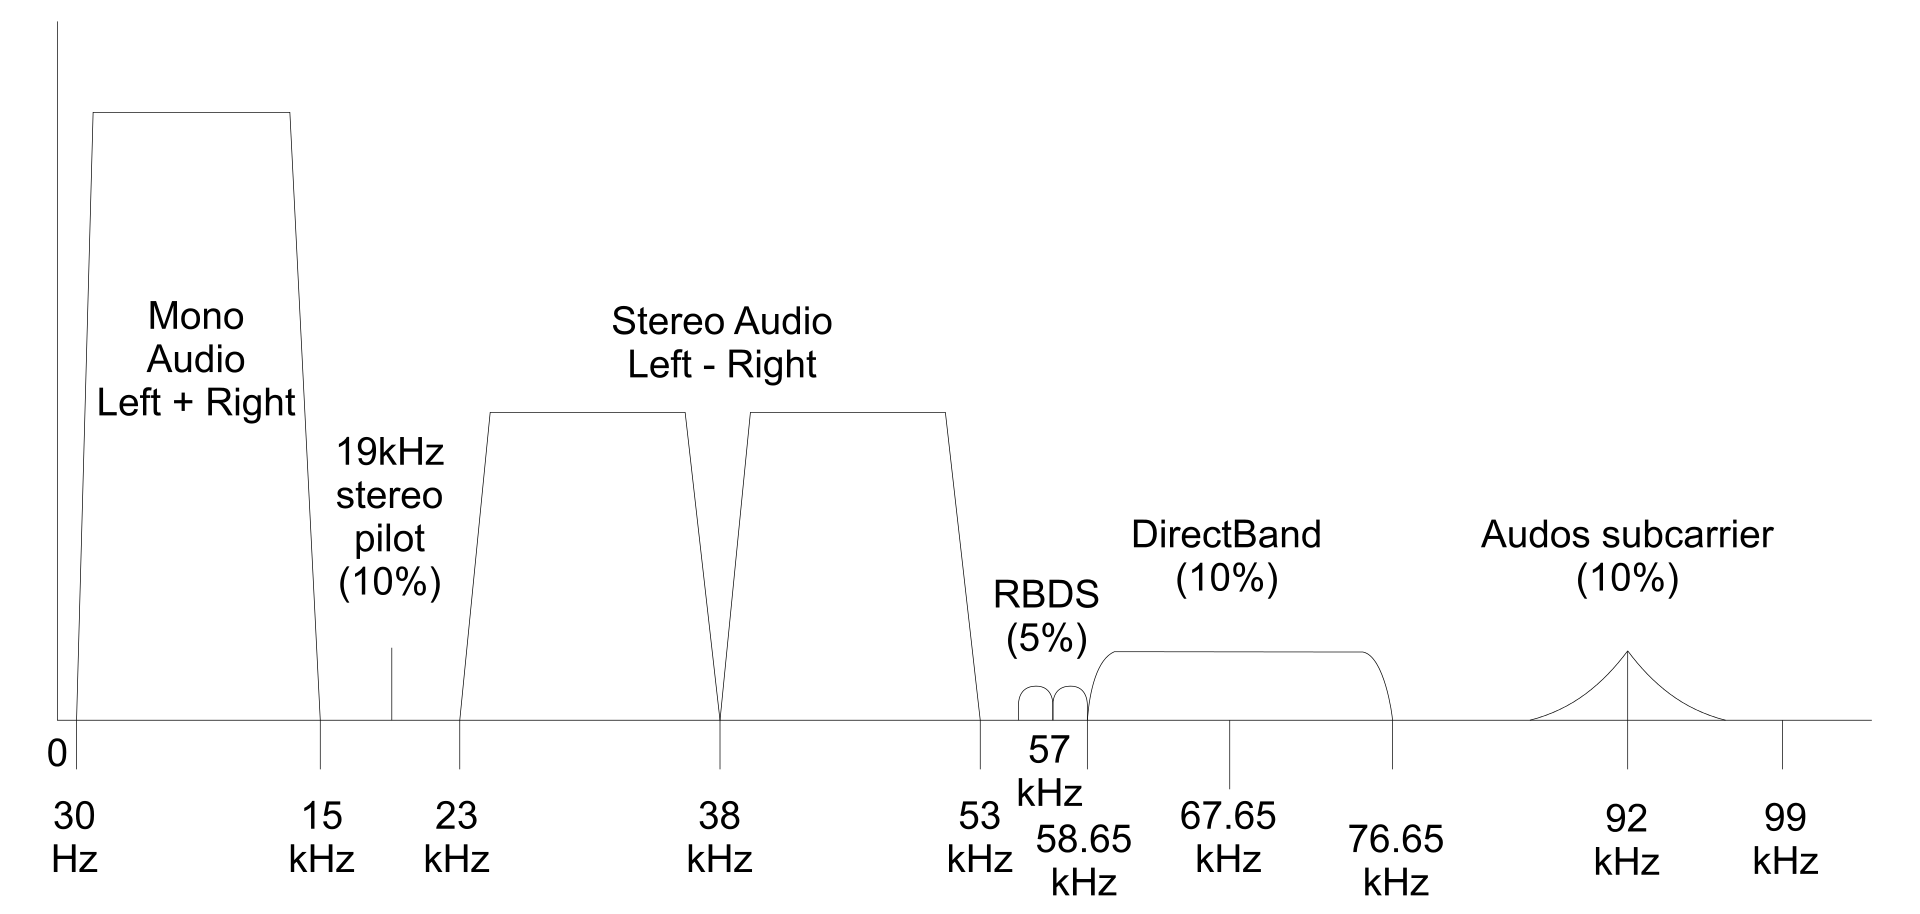
\includegraphics[scale=0.13]{img/RDS_spectrum2}
		\caption{FM broadcast spectrum}}
		\label{fig: spec}
	\end{figure}

	As the illustration displayed the RDS center frequency (FC) is localized at 57kHz and has a 5 percent bandwidth. For a correctly demodulation of the RDS signal, it is important to calibrate the receiver to FC.
	
	Radio stations like O3, Kronehit and FM4 use various FM broadcasting features for example \cite{Stau}. Also, the fire department, the police, the Austrian automobile- motorcycle and touring club (ÖAMTC) and other traffic service agency use the standard \cite{standard}.
	
	An RDS information block contains multiple traffic data \cite{Dietman}: 
	
	\textit{Traffic Programme} (TP) code: Serving to identify programs that, from time to time, carry messages addressed to motorists.
	
	\textit{Traffic Announcement} (TA) signal: Switches a traffic announcement to a preset volume level and, if the motorist is listening to a cassette rather than the radio, stops the cassette and switches the radio on to receive the traffic message instead.
	
	\textit{Emergency Warning System} (EWS): A feature using a very small amount of data for emergency warning services such as national disasters and hazardous chemical spills.
	\\
	
	
	%%% Contribution %%%
	\section{Related Work}
	\todo{Ich weiss nicht ob du dich an meine presentation errinerst, aber da habe ich genau erzählt wofür die section ist. Da soll stehen was andere läute im gleichen feld gemacht haben. Salesman:too informal; this is supposed to be a paragraph on previous work done in your field, not simply a summary of your story}
	For two years I have been working with signal processing in telecommunication orientated embedded systems. Both of these terrestrial broadcasting systems use bit interleaving and bit error forward correction to negate signal loss which will occur during transmission \cite{Terre}. These methods were also used in RDS. In particular a simple receiver with analog to digital converter is the only needed hardware. This hardware is called SDR-stick, Software Defined Radio. Figure \ref{fig: receiver} shows the used set up for RDS receivers.
	
	
	\begin{figure}[h]
		\centering
		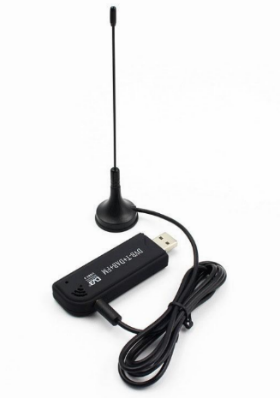
\includegraphics[scale=0.63]{img/SDR-Stick}
		\caption{SDR-Stick \todo{Hier sollst du das bild beschreiben nicht den namen des produkts schrieben. Salesman: readability is an issue here, as it is in Figure 1. As you learned in the course, every visualization is led in and out, described completely and related to the overall narratie, the argument of the paper}}
		\label{fig: receiver}
	\end{figure}
	
	With this setup, various signal processing can be achieved. (RDS and FM stereo radio are some of the main features of  FM broadcasting. This high frequency (HF) receiver could also be used as digital video broadcast receiver) \todo{mark examples as such}. The University of Strathclyde, Glasgow-Scotland, is known as one of the biggest software developers in this field \todo{which?}. The institute \todo{which?} engineered a new algorithm to transmit RDS \cite{stewart2015software}. Many methods such as the costas loop and the sequence of timming recovery have been used in my work.\\
	
	\section{Aim of this Paper}
	\todo{The point in this section is to give aims that can be checked at the end; make sure you pick those up in the conclusion and can serve them with the knowledge created in your paper}
	In this paper I elaborate the application of this broadcast system to prove \todo{Was auch immer}. There is a big potential in in broadcast system utilization in the growing society. (Furthermore, this paper will try to point out)\todo{too colloquial; write more formally in a research paper} the impact these applications have in the current economy of \todo{Western countries oder was anderes...Salesman: see before: which? What can be learned from discussing the implications? What's the point here? Make it clear, already here before you do it. }. The transmission standard Blaupunkt developed in the early eighties has since been adapted into modern technologies. Additional experiments should reflect the versatility of the standard. \todo{Wie in previous work ist das in der falschen stelle. in Aim must du schreiben was du erreichen möchstest, später kkommt der teil wie du es machst, in result welche resultate du bekomment hast und conclusion ob due es erfolgeich geschaft hast oder nicht und wieso. Wenn du etwas nicht schafst und schrreibst wieso ist es gut. In einem scientific writing ist es auch sehr hilfreich für die nächsten die das machen wenn sie aus deinem fehler lernen.}\\		

	%%% Originality & Related Work %%%
	\section{Background of RDS}
	In the early eighties, blaupunkt tried to develop a fast and cheap communication standard for radios \todo{Vieleich sollst du den teil in aim löschen und nur hier lassen, obn hegört es sowieso nicht dazu}. Blaupunkt focused on music information, any radio should be able to receive RDS signals \cite{DietmanRDSbeginning}. The audio engineer’s reference book released the first RDS specification\cite{firstRDSspecEBUTECH}. Including following information:
	
	\textit{List of Alternative Frequencies} (AF): Stereo Audio needs this feature to obtain the nearest transmitter mast
	
	\textit{Clock Time and date} (CT): Time and date synchronization feature.
	
	\textit{Music Speech switch} (MS): An indicator of whether music or speech is broadcasted
	
	\textit{Programme Identification} (PI): A 16-bit code giving a unique serial number to a program service
	
	\textit{Programme Item Number} (PIN): Scheduled start time and date for an individual program
	
	\textit{RadioText}  (RT): Text for display
	
	\textit{Programme Type} (PTY): Identifies the type of the program from a list of 31 possibilities \todo{sie hat recht das hat überhaupt kein informationswert. Schrieb vielleicht die wichtigsten possibilities und wieso se wichtig sind. Salesman: transition here from this information to what comes next; why was this important?}\\
	
	A conventional terrestrial receiver circuit can be utilized to receive the above stated features. DVB-T transmission employs the same terrestrial circuit with the significant difference that there is encryption. Figure \ref{fig: receiverCircut} shows the demodulator for an RDS signal. This module is still applied on modern devices to this day.
	
	\begin{figure}[h]
		\centering
		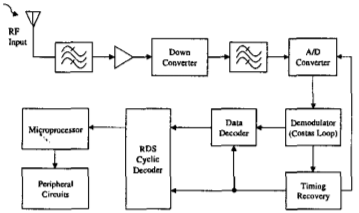
\includegraphics[width = \linewidth]{img/circut}
		\caption{digital circut for RDS receivers}
		\label{fig: receiverCircut}
	\end{figure}
	
	The traffic related features like TA and TP have been added \todo{to radios -> oder was auch immer. ich habe mein mehl hinzugefügt, jemand der nicht weis das man es in wasser zufügt um teig zu bekommen kann nicht mit der info anfangen} in 1990 \cite{TATP}. Traffic Message Channel (TMC) was later implemented into the standard in 2007. This channel made it possible to transmit traffic-related information by broadcasting them digitally. By incorporating TMC, the navigation systems were able to operate in real time  \cite{barca2017radio}. Albeit, the terrestrial transmission method has remained the same since 1983. \todo{Weil es die industrie es nicht nötig hatte oder es kein geld in der forschung gibt oder oder oder....Das gleich wie oben. Kein informationswert. Salesman: and, why is this relevant? explain!}\\
	
	%%% Relevance %%%
	\section{Findings}
	
	The RDS standard did not include encryption for data transmission\todo{wich is necessary in order to achieve safe data transmission. Salesman: when?}. Online tutorials and books describe how the standard works and what equipment is utilized to build a RDS broadcast system. Figure \ref{fig: standard} shows the transmission standard \cite{DIN_EN}. \todo{Salesman: I do not understand what happens from here on out }
	
	
	The implementation of a check in addition to the offset \todo{du hast nicht erklert was ein offset ist} serves a bit recovery purpose only \todo{and can not be used for purposes such as ..... because of .... Versuche das aber in 2 Sätzen zu schreiben}. (Bit recovery and bit check systems are embedded into every HF transmission). \todo{Genau was sie gesagt hat. Salesman: ah, this needs to come before}
	
	\begin{figure}[h]
		\centering
		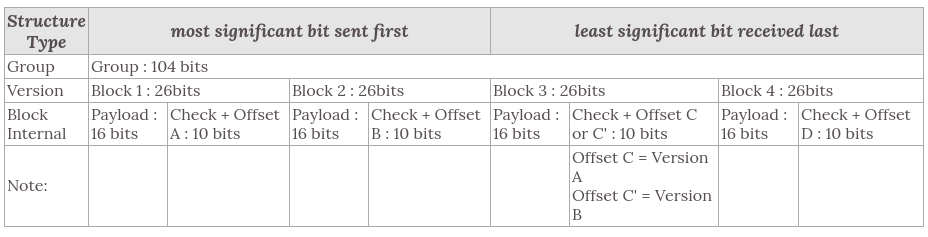
\includegraphics[scale=0.265]{img/standard}
		\caption{RDS transmission standard \todo{Lead into this Figure, describe and explain; again, readability is an issue}}
		\label{fig: standard}
	\end{figure}
	
	Considering the fact that RDS is based on terrestrial broadcast and every HF antenna can receive this signal, the transmission can be intercepted by any host \todo{in order to achieve ... was auch immer Salesman:and? is this an opporunity, a danger, if so why? Explain this}. This standard is still used by the police, the fire department and the ambulance.  Based on the encryption, this standard is not reliable, but must be used by the state regulation in \todo{Austria, Europe, America??}. According to § 89 of the TKG, the malevolent manipulation or interception of their communication is illegal \cite{telecomGesetz}. \todo{Fakten haben keine bedeutung und antworten nie auf die frage wieso. Himmel ist blau. das ist ein fakt, aber dadurch hast du keine idee wieso er blau ist... Mann soll ein statement erkleren. beispielweise könntest du schreiben: Because the standard is not encrypted is makes it vulnerable and the data could easily be retrieved from unwanted persons or institutions. <-- überlege es noch einmal. Salesman: so? You toss in facts; rather, name and explain and create an argument – this is what the course taught you. Remember the four steps and create your text according to them}\\
	
	
	\section{Applications \todo{of broadcasting signals <- oder was halt richtig ist. Applications of?}}
	Information processing is key for any automated system due to the fact that \todo{schreib jetzt wieso es key ist. Salesman: – this is so general that it carries no information; be precise and stick within the space you deal with here}. These systems need input in order to operate properly \todo{Was sie damit sagen wollte ist, welche system brauchen input um wie zu funktionieren? Mit dem toddler hat sie recht, ein baby brauch auch essen (input) um gesund leben zu können (operate properly)... zu generel.. Salesman: again, too generl; this is true for a toddler, too}. For example, self-driving cars rely on information about the road, traffic lights and pedestrian frequency. These conditions are measured by sensors and distributed to various receivers via RDS. For future applications, this standard can be expanded by additional information blocks. Moritz Dechant, senior developer Bosch, claimed in an interview that any external input for self driving cars would lighten the required computing  power \cite{bosch} \todo{Ich wüde das auslassen, das ist nur ein claim kein ultimativer beweis das es so sein wird <- Theoretisch kannst du ihn auch so diskreditieren wenn es anders in der zukunft wird. Wenn du das unbedingt haben wills dann formuliere es anders bsp: Experts in this field are positive about the idea that any external input for self driving cars could potentially lighten the required computing  power <-- so brauchst du keine referent. Salesman: so, how does that connect to the need for information processing you talked about before in this paragraph? }.
	
	\subsection{TP and TMC inpact on traffic} \todo{ <- In latex ist es eine subsection}
	
	Traffic jams are a big issue in european cities like Vienna. For those directly affected, the damage is quantified in loss of time. According to these estimates, every german citizen spends an average of 50 hours a year in traffic jams \cite{Stau}. Lost working hours, traffic-related accidents and fuel consumption amount to a loss in over 100 billion euro. 
	
	To keep the timeloss short as possible, modern navigation systems operate in real time. 
	Various algorithms help drivers find the best route possible using information provided through TMC and TP. This data contains traffic related information about nearby construction sites, congestion and roadblocks \cite{uyeki2010route}.
	
	
	\subsection{Monitoring public transport data}
	
	The princip of data sharing helps to economize the infrastructure in Shanghai. The metropolis utilize the FM standard to record some data about rush hours. The puplic transport with buses are connectet with an TMC server, which can operate in realtime to broadcast some issues. One of the biggest advantages of RDS is that the standard doen't need addinational infrastructure. The already mounted FM radio mast supports the broadcsating of traffic information. Figure \ref{fig: monitoring} illustrate the TMC network \cite{Monitoring-du2014effective}.
	
	\begin{figure}[h]
		\centering
		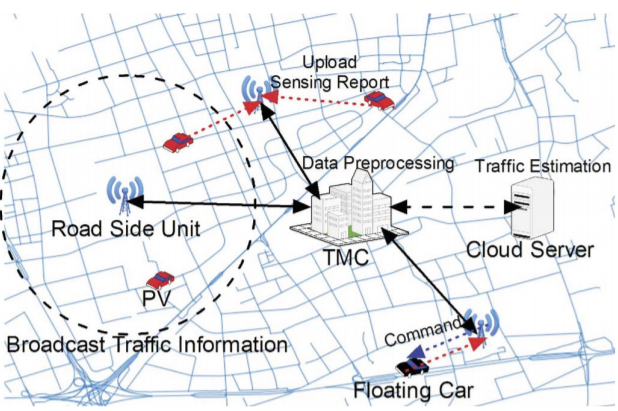
\includegraphics[width =0.5 \linewidth]{img/monitoring}
		\caption{Urban information broadcasting \todo{wie in der obigen figur Salesman: description missing, lead in and lead out, make readable etc.}}
		\label{fig: monitoring}
	\end{figure}
	
	
	\subsection{Pollution}
	
	Bigger cities, like Stuttgart, also uses RDS to collect sensor datas like air polution. Sensor boxes are placed on highly frequented roads to alarm if a certan level of particulate matter. This warning system started in the year 2018 \cite{Stuttgart}.\\			 
	
	
	\section{Experiments with RDS} %%%%%Hierstelen geblieben
	\textbf{RDS of things - Smart City}
	
	In a study \todo{namen! Nicht türkisch, es ist kein essen :P}(2019), a smart city prototype was built which served as the communication channel with the RDS standard. The prototype included traffic lights, emergency services and general traffic flow services. The prototype was also developed with 2G and LoRaWan. The replicated cities were London, New York and Moscow. The results are shown in Figure \ref{fig: smartCity}.The study shows that RDS is a lot cheaper. Furthermore, the introduction is also cheaper because the existing transmission masts can be reused \cite{SmartCity-kutlay2019rds}.
	
	\begin{figure}[h]
		\centering
		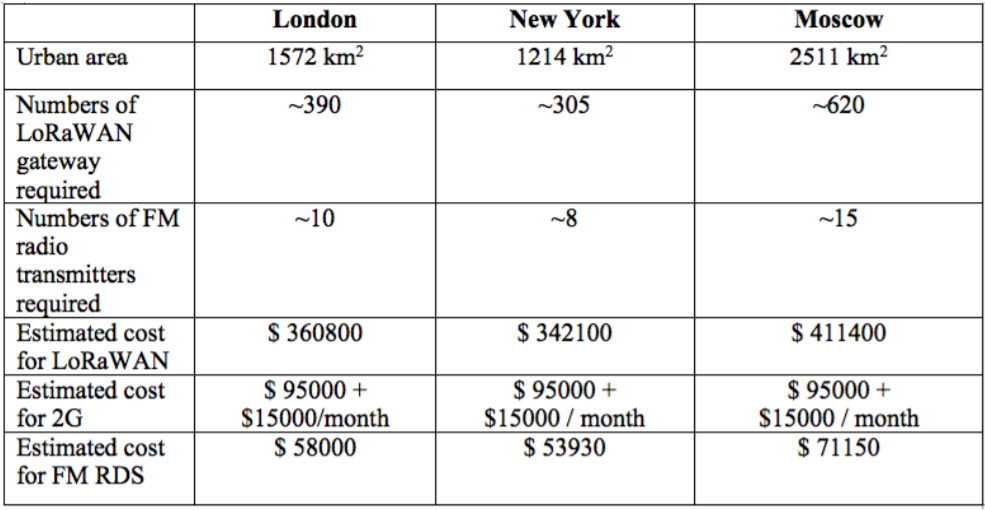
\includegraphics[width = \linewidth]{img/smartCity}
		\caption{Comparesing RDS with 2G and LoRanWan}
		\label{fig: smartCity}
	\end{figure}
	
	\subsection{Health monitoring using Radio Data Systems}
	
	In order to reduce the costs and ooccupancy \todo{ich weis nicht was das bedeutet sry.. }rate of hospitals, a monitoring system has been presented by R.S. Deepak Ram in a studies. This system consists of one health control unit and an central that receives the health data. The health control unit indicates condition where a hospital treatment is needed and omit this information to the nearest central. RDS is implemented as communication standard in this experiment. According to the publisher of this experiment one problem is highlighted, the secure level of the system is based on FM broadcast \cite{Healthcare-ram2015health}. \\
	
	
	
	\section{Impact of an insecure standard}
	
	A study shows that 95 percent of the drivers trust their navigation system \cite{trustNavi_stanton2014advances}. Considering that the standard is not encrypted it gives space to manipulate the data broadcast. If a person has the intention to cause a traffic jam, by manipulation the RDS broadcasting, they will face no technical obstacles to fake information. 
	
	The TU traffic planer Hermann Knoflacher gained unpopularity after he deliberately caused congestions to reduce the amount of commuters driving through Vienna.
	He strategically placed some construction sites on busy roads to form multiple traffic jam\cite{presse}. As a reaction to this, navigation systems tried to avoid those streets and thus commuters chose to drive around vienna rather than through it. This same result can be achieved by hackers utilizing RDS. By sharing wrong information on TMC and TP about certain streets, there could be an increase or decrease in the frequency that streets are used. As a consequence, streets could reach maximum capacity and start to congest.\\
	
	
	\section {Conclusion}
	\todo{There is so much more substantial discussion that is needed here; this result did not need research done on the matter}
	
	One of the greatest benefits of RDS is the simple implementation and the low-price setup. Existing FM radio transmission masts are reused for current applications. Even more features can be broadcasted within the RDS signal without changing the infrastructure. This is possible thanks to the broader FM frame of the RDS. This paper illustrated some versatile application where data sharing via RDS can optimize the infrastructure. Considering the fact that the standard has no encryption, it should not be integrated as a carrier of sensible data eg. medical and financial information. 
	
	The consequence of keeping the standard is to take the risk of being hacked, but it is a small price to pay, considering the low costs of the current systems. 
	
	
	%%%%%%%%%% BIBLIOGRAPHY %%%%%%%%%%%%%%%%%%%%%%%%%%%%%%%%%%%%%%%%%%%%%%%%
	\bibliographystyle{IEEEtran}
	\bibliography{bibliography}
	%%%%%%%%%%%%%%%%%%%%%%%%%%%%%%%%%%%%%%%%%%%%%%%%%%%%%%%%%%%%%%%%%%%%%%%%
\end{document}